\documentclass[12pt,a4paper]{article}
\usepackage{geometry}
\geometry{left=2.5cm,right=2.5cm,top=2.0cm,bottom=2.5cm}
\usepackage[english]{babel}
\usepackage{amsmath,amsthm}
\usepackage{amsfonts}
\usepackage[longend,ruled,linesnumbered]{algorithm2e}
\usepackage{fancyhdr}
\usepackage{ctex}
\usepackage{array}
\usepackage{listings}
\usepackage{color}
\usepackage{graphicx}
\usepackage{amssymb}
\newtheorem{theorem}{定理}
\newtheorem{lemma}[theorem]{引理}
\newtheorem{corollary}[theorem]{推论}

\begin{document}
	
	\noindent
	
	\section*{2024.04.22}	
	
	\begin{enumerate}
		\item 证明如下引理.
		
		设$P_k$是$d$维空间,$\{N_1,\cdots,N_L\}$是$P_k$的对偶空间$(P_k)^{\prime}$的一个子集. 则下面两个条件等价
		
		(a) $\{N_1,\cdots,N_d\}$是$(P_k)^{\prime}$的一组基
		
		(b) 对任意$\phi\in P_K$,$N_i(\phi)=0,1\leq i\leq d$等价于$\phi\equiv0.$
		
		\begin{proof}[证明]
			令 $\{\phi_1, \ldots , \phi_d\} $ 为 $P_k$ 的一组基.$\left\{N_1,\ldots,N_d\right\}$ 是 $P_k^{\prime}$ 的一组基当且仅当对于 $\mathcal{P} ^{\prime}$ 中的任意 $L$,
			
			\begin{equation}
				L=\alpha_1N_1+\ldots+\alpha_dN_d  \label{linear}
			\end{equation}
			
			因为 $d= \dim P_k = \dim P_k ^{\prime}$. 式\eqref{linear}等价于
			
			\begin{equation}
				\begin{aligned}
					y_i &:= L(\phi_i) \\
					&= \alpha_1N_1(\phi_i)+\ldots+\alpha_dN_d(\phi_i),\quad i=1,\ldots,d.
				\end{aligned}
			\end{equation}
			
			
			令 $B=\left(N_j(\phi_i)\right),i,j=1,\ldots,d.$ 因此,(a) 等价于 $B\alpha=y$ 有解,即$B$可逆。
			
			对于 $\mathcal{P}$ 中的任意 $v$,我们可以写成 $v=\beta_1\phi_1+\ldots+\beta_d\phi_d.~N_iv=0$ 意味着 $\beta_1N_i(\phi_1)+\ldots+\beta_dN_i(\phi_d)=0.$ 因此,(b) 等价于
			
			\begin{equation}
				\beta_{1}N_{i}(\phi_{1})+\ldots+\beta_{d}N_{i}(\phi_{d})=0\quad\forall i=1,\ldots,d\\\Longrightarrow\beta_{1}=\ldots=\beta_{d}=0.
			\end{equation}
			
			令 $C=\begin{pmatrix}N_i(\phi_j)\end{pmatrix},\:i,j=1,\ldots,d.$ 那么 (b) 等价于 $Cx=0$ 只有零解,即$C$可逆。
			
			由于 $C=B^T$, (a) 等价于 (b).
			
		\end{proof}
		\item 利用网格生成软件包给出L型区域$\Omega=(-1,1)^2\backslash[0,1]\times[-1,0]$的一个
		三角形剖分,画出剖分图(例如gmsh,distmesh等)
		
		\begin{figure}[ht]
			\centering
			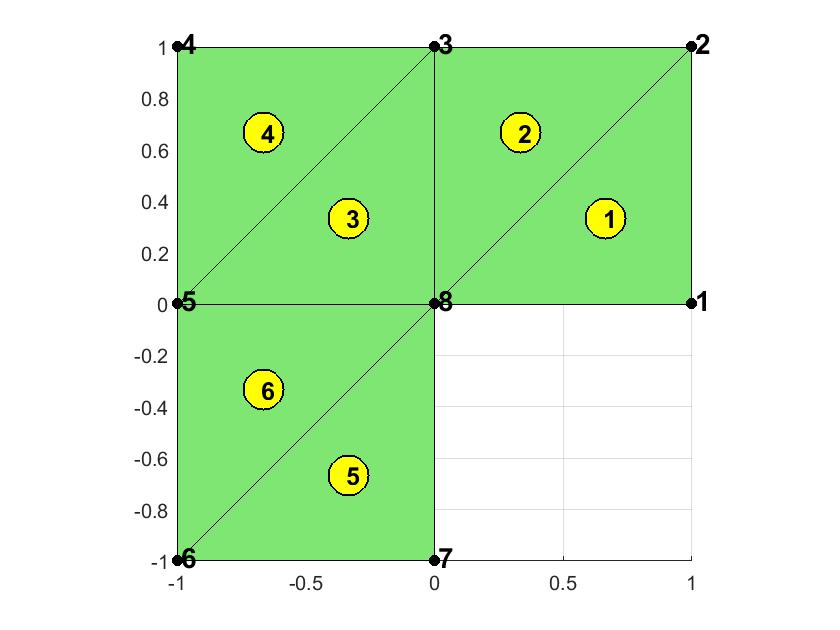
\includegraphics[width=0.8\textwidth]{hw3_2.jpg}
			\caption{网格图}
			\label{fig:triangelmesh}
		\end{figure}
		
		\item 验证
		$$
		\phi_i=\lambda_i(2\lambda_i-1),\quad1\leq i\leq3
		$$
		
		$$
		\phi_4=4\lambda_2\lambda_3,\:\phi_5=4\lambda_3\lambda_1,\:\phi_6=4\lambda_1\lambda_2
		$$
		
		是Lagrange二次元节点基函数. 
		
		\begin{proof}
			直接代入计算可得
			$$
			\phi_1(z_i)=\lambda_1(2\lambda_1-1)=0(2*0-1)=0, \quad i = 2,3,4
			$$
			$$
			\phi_1(z_i)=\lambda_1(2\lambda_1-1)=\frac{1}{2}(2*\frac{1}{2}-1)=0, \quad i = 5,6
			$$
			$$
			\phi_1(z_i)=\lambda_1(2\lambda_1-1)=1(2*1-1)=1, \quad i = 1
			$$
			$$
			\phi_4(z_i)=4\lambda_2\lambda_3=4*0*0=0, \quad i = 1
			$$
			
			$$
			\phi_4(z_i)=4\lambda_2\lambda_3=4*\frac{1}{2}*0=0, \quad i = 5,6
			$$
			
			$$
			\phi_4(z_i)=4\lambda_2\lambda_3=4*1*0=0, \quad i = 2,3
			$$
			
			$$
			\phi_4(z_i)=4\lambda_2\lambda_3=4*\frac{1}{2}*\frac{1}{2}=1, \quad i = 4
			$$
			由对称性以及Lagrange元定义,可得$N_i(\phi_j)=\delta_{ij}$,从而$\phi$是Lagrange二次元节点基函数
		\end{proof}
		
		\item 证明如下定义的Hermite空间属于$H^1(\Omega)$
		
		$$
		V_h=\{v\in L^2(\Omega)\mid v|_K\in P_3(K),\forall K\in \mathcal{T}_h,v\text{在}\mathcal{T}_h\text{的所有顶点连续},\nabla v\text{在}\mathcal{T}_h\text{的所有顶点连续}\}
		$$
		
		(Hint:要证$V_h\subset H^1(\Omega)$只需证在公共边$F=K_1\cap K_2$上,$v|_{K_1}=v|_{K_2})$
		
		\begin{proof}[证明]
			考虑$v|_{K_1}$与$v|_{K_2}$在$K_1\cup K_2$上的延拓,仍记为$v|_{K_1},v|_{K_2}$.
			
			记$w := v|_{K_1}-v|_{K_2}$,则$w$是定义在$K_1\cup K_2$上的$P_3$的多项式.
			
			记$L := K_1\cap K_2$的两个端点为$z_1,z_2$,根据$V_h$定义,有
			$$
			w(z_1)=w_(z_2)=0
			$$
			$$
			w_{L}^{\prime}(z_1)=w_{L}^{\prime}(z_2)=0
			$$
			从而有$w|_{L}\equiv0$. 即$v|_{K_1}=v|_{K_2}$
		\end{proof}
		
		\item 证明如下定义的Argyris空间属于$H^2(\Omega)$ 
		$$V_h=\{v\in L^2(\Omega)\mid v|_K\in P_5(K),\forall K\in \mathcal{T}_h,v\text{和其一阶以及二阶导数在}\mathcal{T}_h
		\text{的所有顶点连续,在}$$
		$$\mathcal{T}_h\text{的所有边中点,}v\text{关于该边的法向导数连续}\}$$
		
		(Hint:要证$V_h\subset H^2(\Omega)$只需证在公共边$F=K_1\cap K_2$上,$v|_{K_1}=v|_{K_2}$, $\nabla v|_{K_1}=\nabla v|_{K_2})$
		
		\begin{proof}[证明]
			考虑$v|_{K_1}$与$v|_{K_2}$在$K_1\cup K_2$上的延拓,仍记为$v|_{K_1},v|_{K_2}$.
			
			记$w := v|_{K_1}-v|_{K_2}$,则$w$是定义在$K_1\cup K_2$上的$P_5$的多项式.
			
			记$L := K_1\cap K_2$的两个端点为$z_1,z_2$,中点为$z_0$,根据$V_h$定义,有
			$$
			w(z_1)=w_(z_2)=0
			$$
			$$
			w_{L}^{\prime}(z_1)=w_{L}^{\prime}(z_2)=0
			$$
			$$
			w_{L}^{\prime\prime}(z_1)=w_{L}^{\prime\prime}(z_2)=0
			$$
			从而有$w|_{L}\equiv0$,进而$w_L^\prime|_L=0$.
			
			考虑$\frac{\partial}{\partial n} v|_{K_1}$与$\frac{\partial}{\partial n} v|_{K_2}$在$K_1\cup K_2$上的延拓,仍记为$\frac{\partial}{\partial n} v|_{K_1},\frac{\partial}{\partial n} v|_{K_2}$.
			
			记$r:=\frac{\partial}{\partial n} v|_{K_1}-\frac{\partial}{\partial n} v|_{K_2}$,则$r$是定义在$K_1\cup K_2$上的$P_4$的多项式.
			
			根据$V_h$定义,有
			
			$$r(z_1)=r(z_2)=r(z_0)=0$$
			$$r_L^\prime(z_1)=r_L^\prime(z_2)=0$$
			
			从而有$r|_{L}\equiv0$.
			
			结合上述讨论,可得$v|_{K_1}=v|_{K_2}$ , $\nabla v|_{K_1}=\nabla v|_{K_2}$
		\end{proof}
	\end{enumerate}
	
	
\end{document}

